\documentclass[12pt]{report}
\usepackage[margin=1in]{geometry}
\usepackage{setspace} % for single/doublespacing commands
\usepackage{graphicx} % including graphics
\usepackage{sectsty} % sexy section headings
\usepackage[export]{adjustbox} % for graphic frames and center
\usepackage{siunitx}
\usepackage{lmodern} % font package for above
\usepackage[justification=centering]{caption} % figure captions (force centering)
\usepackage{enumitem} % add arguments for enumerate to change style
\usepackage[list=true]{subcaption} % subfigures with list of figure support
\usepackage{multirow}
\usepackage{booktabs}
\usepackage{color}
\usepackage{ulem}
\usepackage[numbers]{natbib}
\usepackage{contour}
\usepackage{tabularx}
\usepackage{framed}
\usepackage{amssymb} % special math symbols
\usepackage{listings}
\usepackage{array}
\usepackage{fancyhdr}
\usepackage{color, colortbl}
\usepackage{tocloft}
\usepackage{url}
\usepackage{etoolbox}
\usepackage{hyperref}
\usepackage{tikz}
\def\checkmark{\tikz\fill[scale=0.4](0,.35) -- (.25,0) -- (1,.7) -- (.25,.15) -- cycle;}
% \setlength{\parskip}{\baselineskip}%
\setlength{\parindent}{0pt}%
\setcounter{secnumdepth}{5}
\renewcommand{\bibname}{References}
\sisetup{output-exponent-marker=\ensuremath{\mathrm{e}}}
\newcommand{\PreserveBackslash}[1]{\let\temp=\\#1\let\\=\temp}
\newcolumntype{C}[1]{>{\PreserveBackslash\centering}p{#1}}
\newcolumntype{R}[1]{>{\PreserveBackslash\raggedleft}p{#1}}
\newcolumntype{L}[1]{>{\PreserveBackslash\raggedright}p{#1}}
\lstMakeShortInline[style=Matlab-editor]| % matlab inline escape character
\graphicspath{{images/}}
\renewcommand\thesection{\arabic{section}}
\renewcommand\labelitemi{---}
\lstset{numberstyle=\ttfamily\small\color{gray}}

\apptocmd{\sloppy}{\hbadness 10000\relax}{}{}
\setlength{\cftbeforetoctitleskip}{-2em}
\allsectionsfont{\raggedright}
\setlist[enumerate]{wide=0pt, widest=99,
                    leftmargin=\parindent,topsep=0pt,partopsep=0pt,
                    label=\thesubsubsection.\alph*,font=\itshape}



\begin{document}
\normalem
\begin{titlepage}
\flushleft
\doublespacing
\Large
\textsc{Test Document} \\
\normalsize
Trey Dufrene, Zack Johnson, David Orcutt, Alan Wallingford, Ryan Warner
\vfill
\center
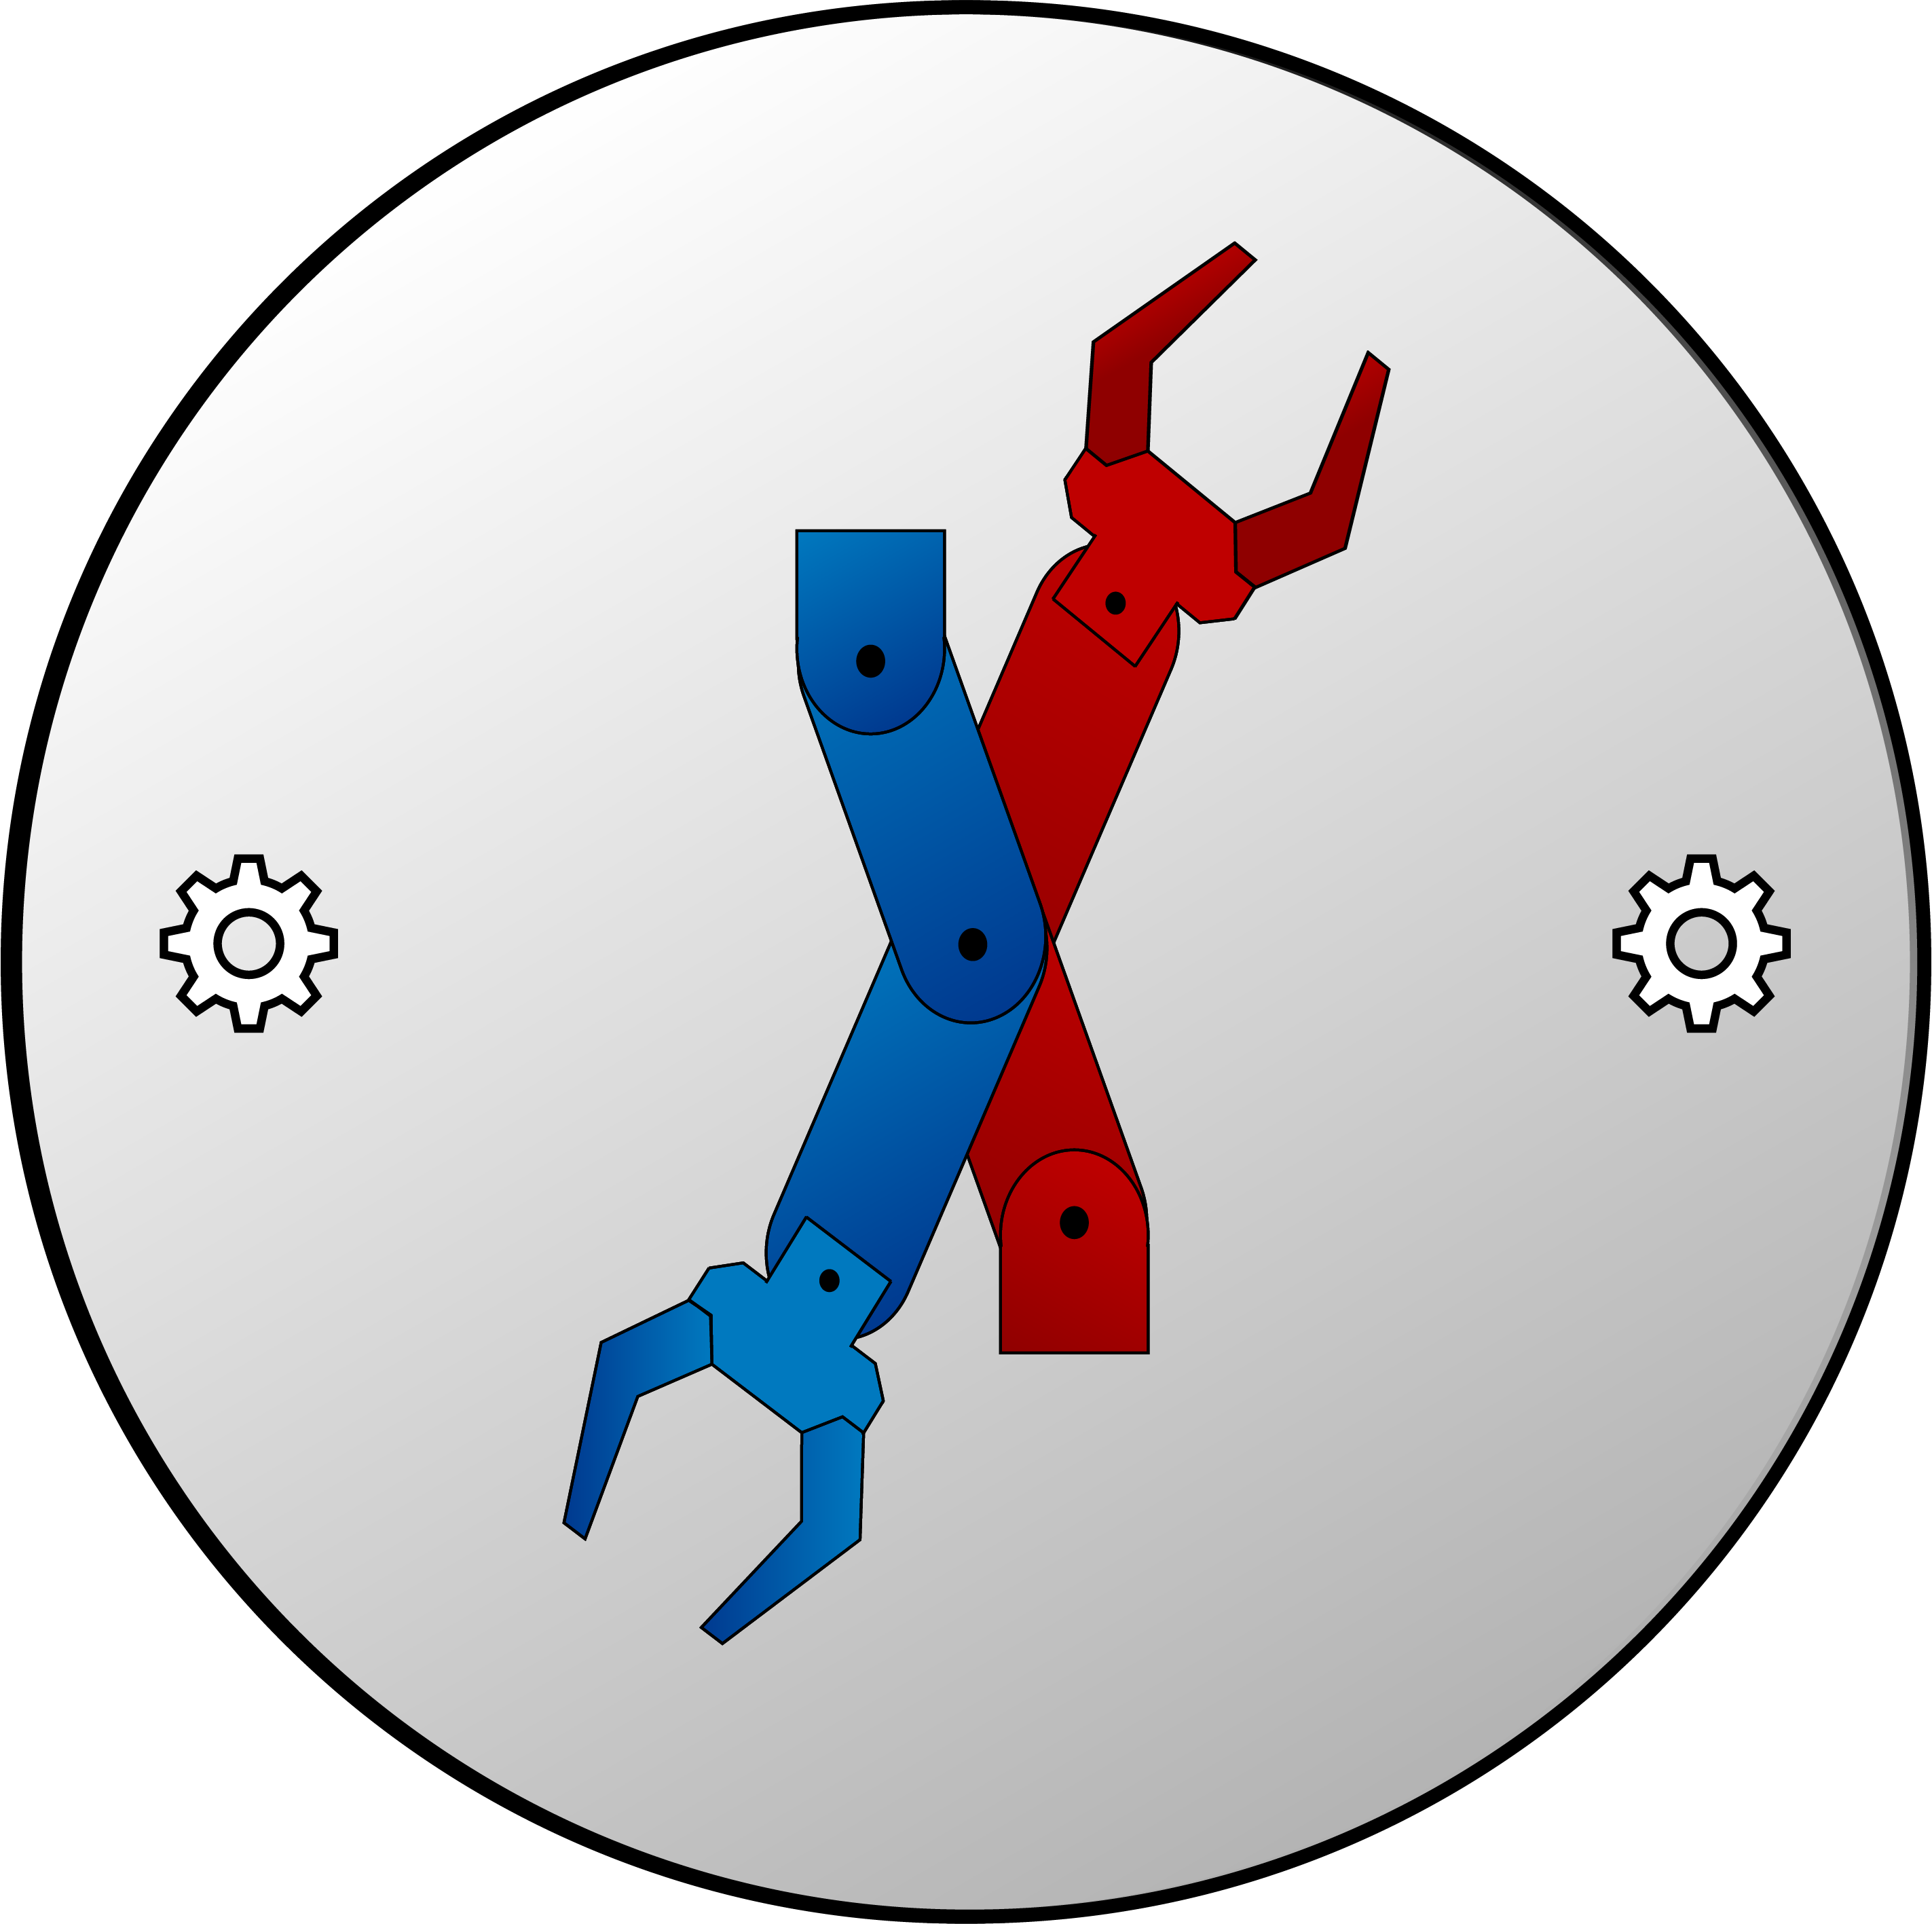
\includegraphics[width=.45\textwidth]{logo}
\vfill
\flushleft
ME 407 \\
Preliminary Design of Robotic Systems \\
Embry-Riddle Aeronautical University \\
\vspace{2ex}
\begin{minipage}[c]{.5\textwidth}
\flushleft

\includegraphics[width=.95\textwidth]{erau}
\end{minipage}%
\begin{minipage}[c]{.5\textwidth}
\flushright

\includegraphics[width=.8\textwidth]{text}
\end{minipage}
\end{titlepage}

\pagenumbering{roman}
% \begin{abstract}
  % Wordy words
% \end{abstract}
{\tableofcontents\let\clearpage\relax\listoffigures}
\clearpage
\newpage
\pagenumbering{arabic}
\raggedright
\section{Introduction}\label{sec:intro}
\section{Specifications and Tests}\label{sec:tests}
Specification \textbf{1.1.a} states: \textbf{The cost for the MEIOSIS team to develop the manipulator shall cost no more than \$800.} This is met if the cost for the MEIOSIS team to develop the manipulator does not exceed \$800. This can be tested by looking at the parts list provided in the parts list seen in Table \ref{tab:bom}.

\begin{table}[htp]
  \centering
  \caption{MEIOSIS Bill of Materials with Costs}
  \label{tab:bom}
  \begin{tabular}{c|c}
      money & money\\
  \end{tabular}
\end{table}

As can be seen in Table \ref{tab:bom}, the manipulator will cost XX and the manipulator meets specification 1.1.a.

Specification \textbf{1.2.a} states: \textbf{The system shall consist of six rotational joints connected by four links. The last three joints will create a spherical wrist.} For this specification to be met, the robot must have six rotational joints and 4 links. The last three joints must create a spherical wrist where the axis of revolution for the last three joints are intersecting with one another. To perform a test to check for six rotational joints, SolidWorks is required. A render of the manipulator with labeled joints can be seen in Figure \ref{fig:manip}.


\begin{figure}[htp]
  \centering
  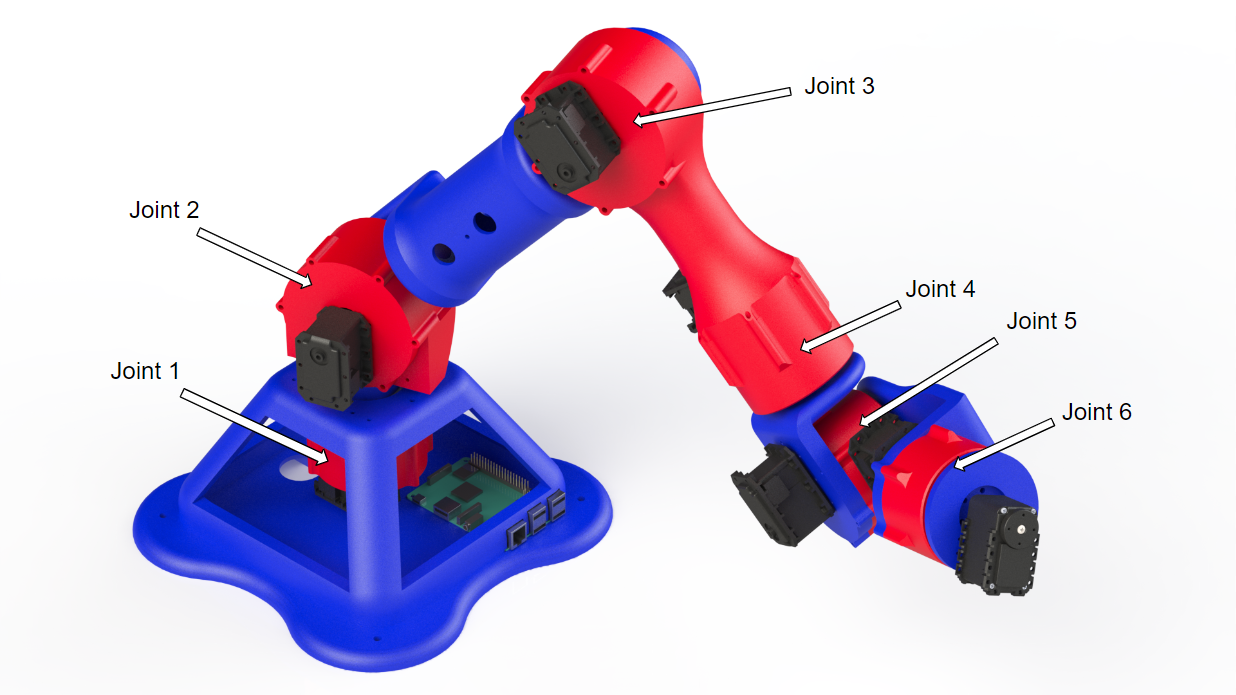
\includegraphics[width=.75\textwidth,frame]{manip}
  \caption{Labeled Image of Manipulator Render}
  \label{fig:manip}
\end{figure}

As can be seen labeled in Figure 1, the robot consists of six rotational joints. Joint 1 controls the rotation about the base,  joints 2-3 control the “shoulder” and “elbow” of the robot, and joints 4-6 control the  spherical wrist. The rotational axis of joint 4 intersects with joint 5’s and joint 5’s also intersects with joint 6’s rotational axis. To perform this test, the assembly file containing the manipulator was opened and the joints were counted. Using the move tool, each joint can be observed to be purely rotational. The data obtained is purely simulated due to the fact that the robot has not been fully fabricated. \textbf{This manipulator meets specification 1.2.a}.

Specification \textbf{1.2.b} states: \textbf{The system shall have no link offsets.} For this specification to be satisfied, there must be no link offsets present in the design of the robotic manipulator. This means that the link should connect two joints by translating in only one direction and the axes of the joints attached to the link should be collinear with one another. Testing this specification requires SolidWorks’ measurement tool. Using the measurement tool, measure each joint to ensure that there is only displacement along one axis. Figure \ref{fig:loff} shows an example of a measurement done on the elbow link of the manipulator.

\begin{figure}[htp]
  \centering
  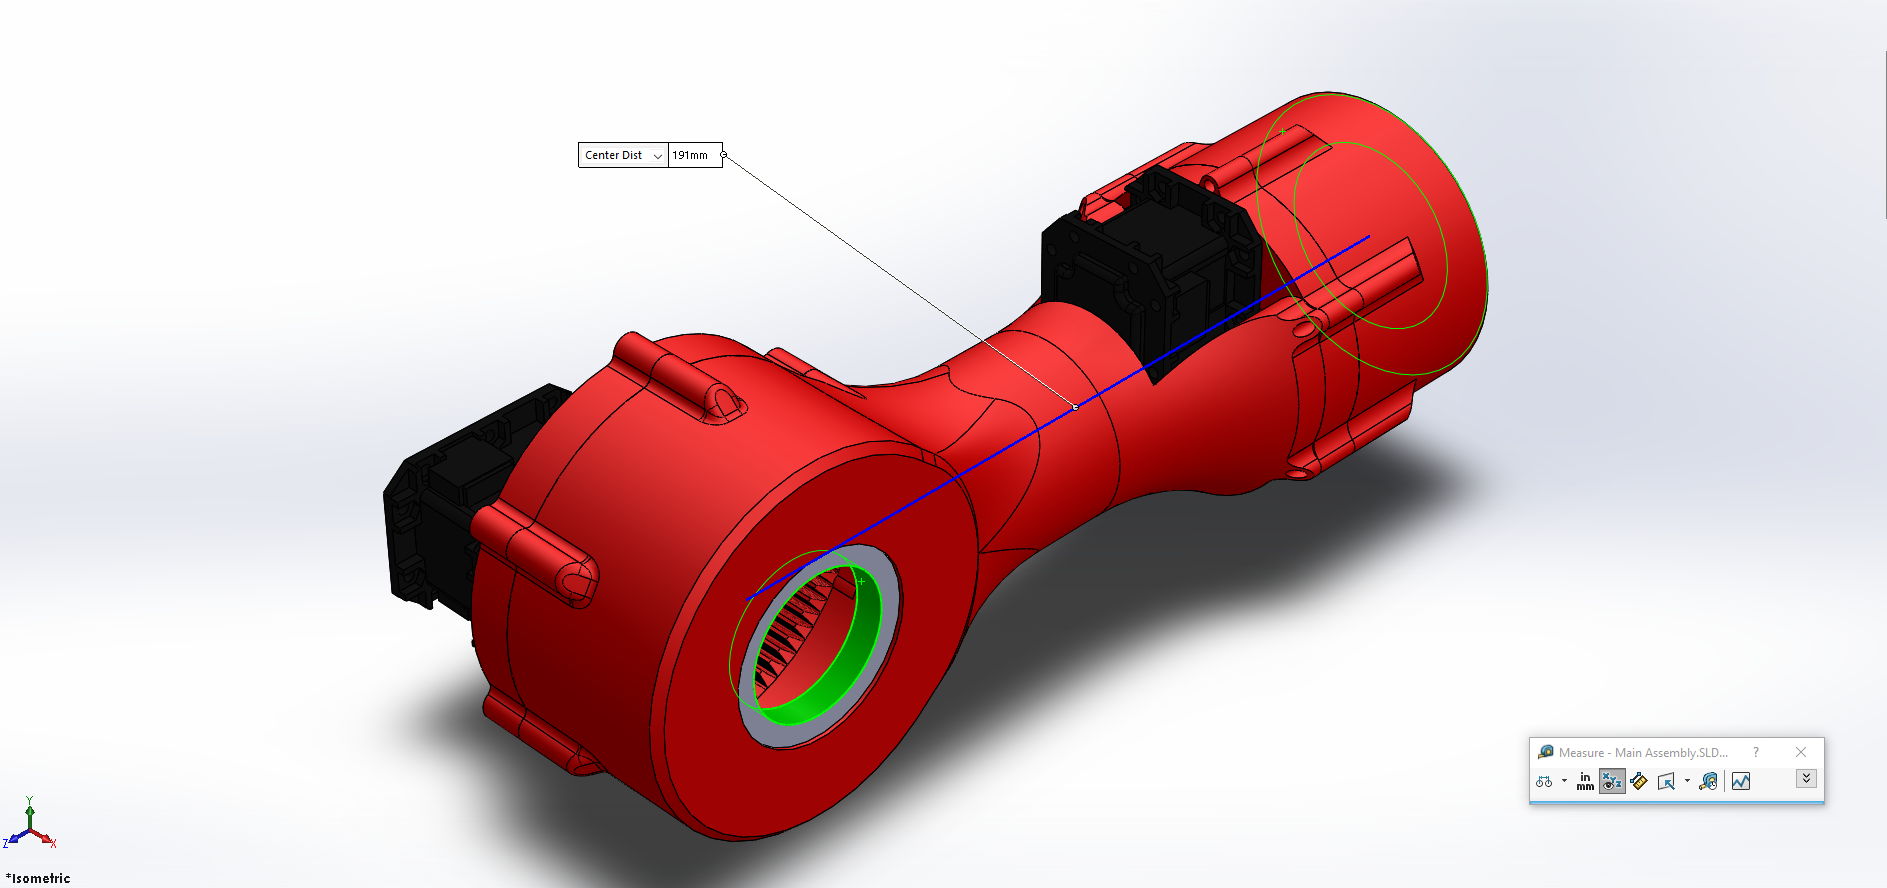
\includegraphics[width=.75\textwidth,frame]{loff}
  \caption{Measurement Test for Link Offset}
  \label{fig:loff}
\end{figure}

Figure \ref{fig:loff} shows a screen capture of a measurement taken and as can be seen by the blue line, the link only extends across one axis. If there were a link offset present, there would be multiple multi-colored lines to show displacement in multiple directions. These tests were done in simulation on each link of the manipulator and none contained any offset direction. Through this test, it is observed that \textbf{the manipulator meets specification 1.2.b}.

Specification 1.3.a states: The system shall accommodate a process in which the end user can calibrate the end effector position and orientation to within 0.5 mm and 1 degree of the manipulator’s precision. In order to fulfill specification 1.3a, an algorithm was developed for calibration. This algorithm must allow the user to manually move the links into a desired zeroed configuration, then accurately retain that zeroed configuration as a reference position during use. Figure 3 depicts the manipulator in a zeroed configuration.

\section{Conclusion}\label{sec:conc}

\begin{table}[htp]
  \centering
  \caption{Summary of Test Results}
  \label{tab:results}
  \begin{tabular}{c|c}
  Specification Tested & Specification Met? \\ \hline
  1.1.a & \\
  1.2.a & \checkmark \\
  1.2.b & \checkmark \\
  1.3.a & Cannot be Determined \\
  1.4.a & Cannot be Determined \\
  1.4.b & Cannot be Determined \\
  1.4.c & Cannot be Determined \\
  1.5.a & \checkmark \\
  1.5.b & \checkmark \\
  1.6.a & \checkmark \\
  1.6.b & $\times$ \\
  1.7.a & \checkmark \\
  1.7.b & Cannot be Determined \\
  1.8.a & Cannot be Determined \\
  2.1.a & \\
  2.2.a & \\
  2.2.b & \checkmark \\
  \end{tabular}
\end{table}
\newpage
\appendix
\renewcommand\thesection{\Roman{section}}
\renewcommand\thesubsection{\roman{subsection}}
\section*{Appendix}\label{sec:app}


\newpage
\bibliographystyle{plainnat}
\bibliography{robo}


\end{document}
